\chapter{Storage}
\begin{sidenotebox}{Great Exceptions!}
    There are exceptions to many of the rules, implementation details discussed in this course. Most of the good (and bad) ideas considered here have been implemented several ways.
\end{sidenotebox}

\section{Database Management System Kernel}
\begin{center}
    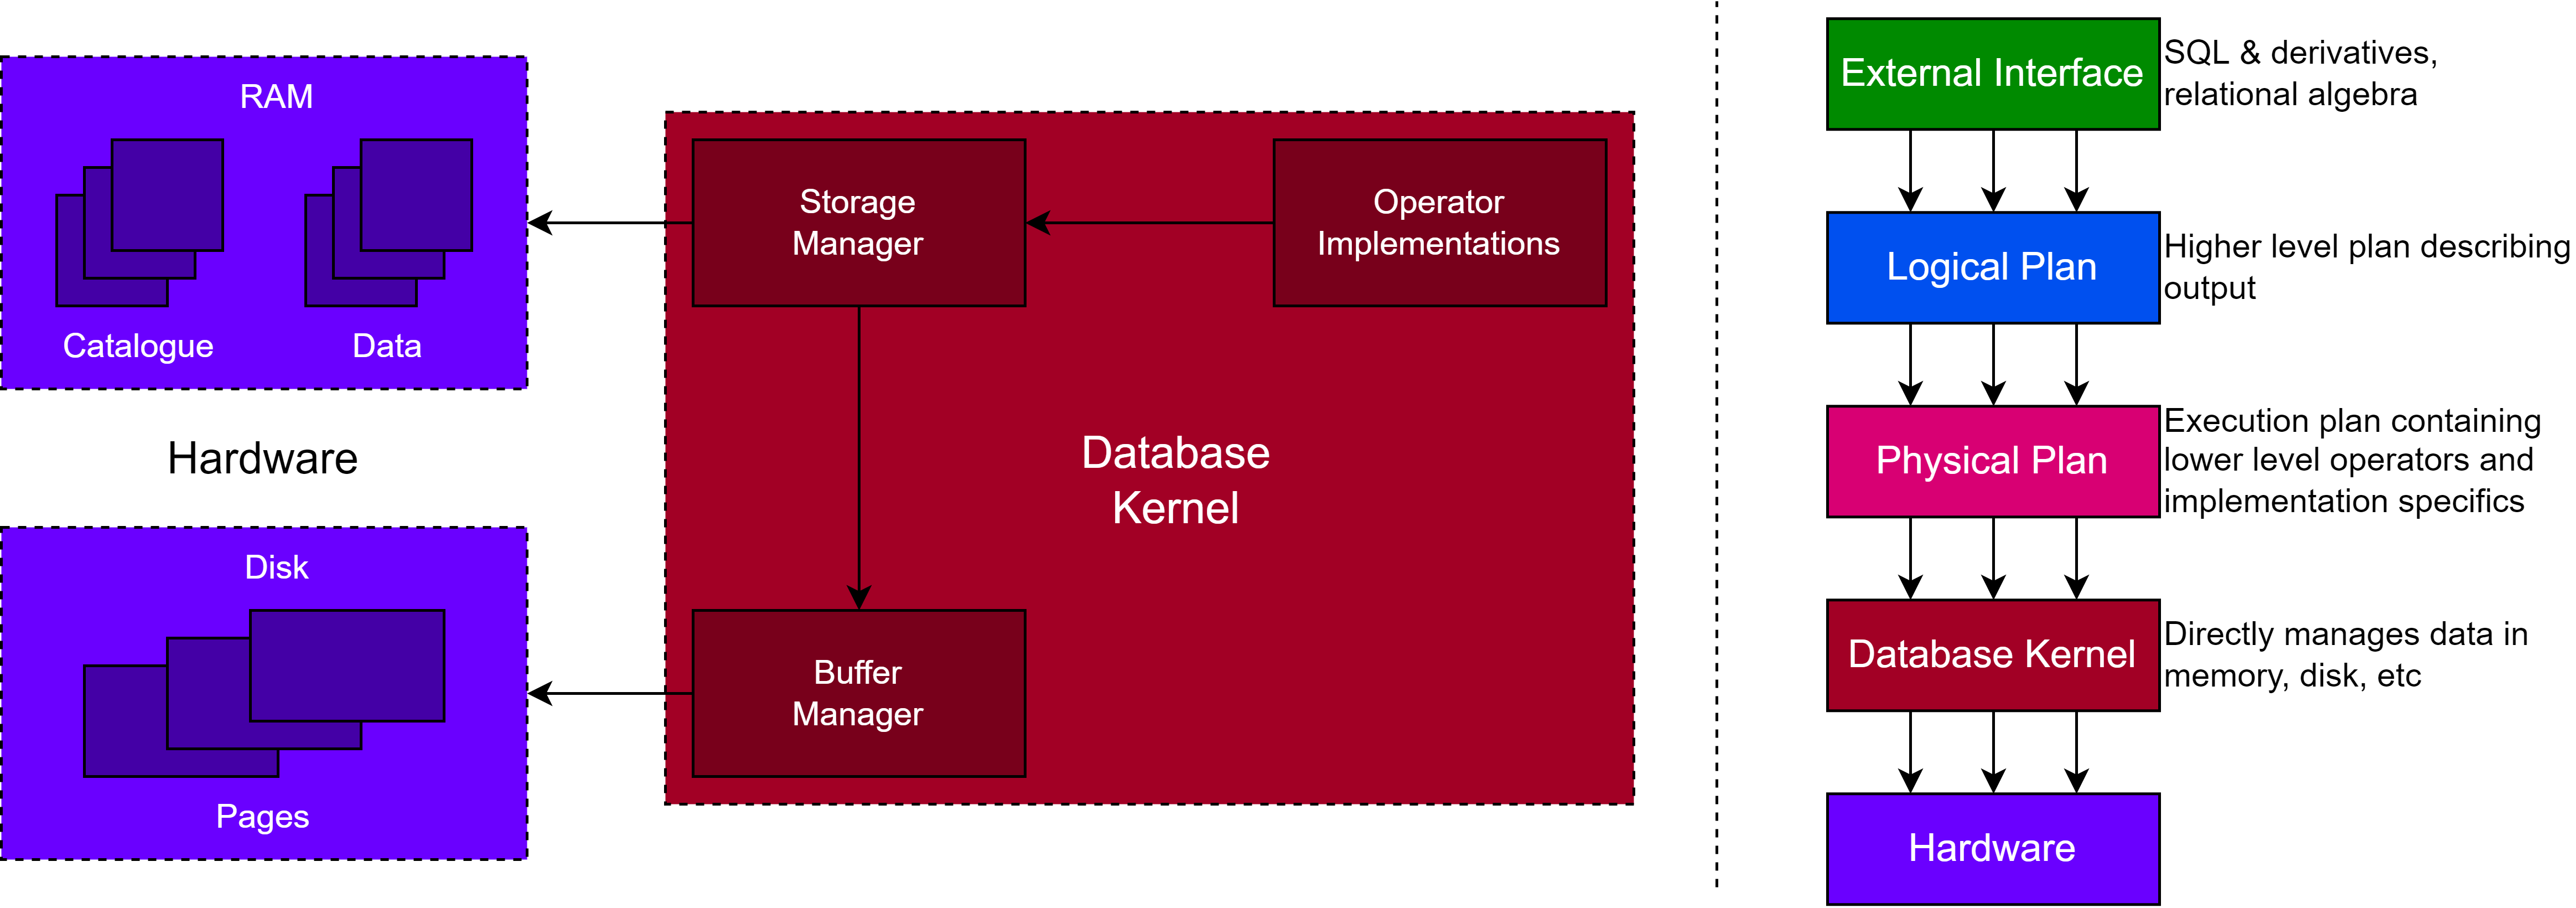
\includegraphics[width=.8\textwidth]{storage/images/kernel_architecture.drawio.png}
\end{center}

\begin{definitionbox}{Database Kernel}
    The core of the database management system.
    \begin{itemize}
        \item Manages interaction with hardware (e.g I/O, memory management, operations)
        \item Library of functionality that implements physical plan \& upwards.
        \item Provides an interface to access subsystems
    \end{itemize}
    Many often bypass the operating system to implement functionality usually associated with OS kernels.
\end{definitionbox}

\section{Storage}
\subsection{Storage Manager}
Multi-dimensional data must be stored in a 1-dimensional memory.
\begin{itemize}
    \item Here we assume the tuples contain data types of a fixed size.
    \item Access latency of memory is determined by cache, hence locality is a key consideration.
    \item We need to consider the access pattern.
    \item Tables are externally represented as a set of tuples.
    \item We assume no concurrency for simplicity here.
\end{itemize}

\begin{sidenotebox}{Optimising for Cache}
    The \href{\ACAURL}{60001 - Advanced Computer Architecture} module by Prof Paul Kelly covers caches and access latency in great depth.
\end{sidenotebox}
\begin{definitionbox}{Locality}
    Average memory access latency is reduced using multiple levels of caches. These caches are designed to take advantage of locality in memory accesses within a program.
    \begin{center}
        \begin{tabular}{l p{.2\textwidth} p{.6\textwidth}}
            \textbf{Spatial} & Accessing nearby/contiguous locations. & A cache miss on a word results in entire line (typically larger than a word) begin cached. Hardware prefetchers fetch lines adjacent to misses. \\ 
            \textbf{Temporal} & Accessing the same location. & Lines stay until evicted due to capacity or flush, load-store queues effectively cache resent accesses. \\
        \end{tabular}
    \end{center}
\end{definitionbox}


\begin{definitionbox}{N-ary Storage}
    Tuples are stored adjacently.
    \begin{center}
        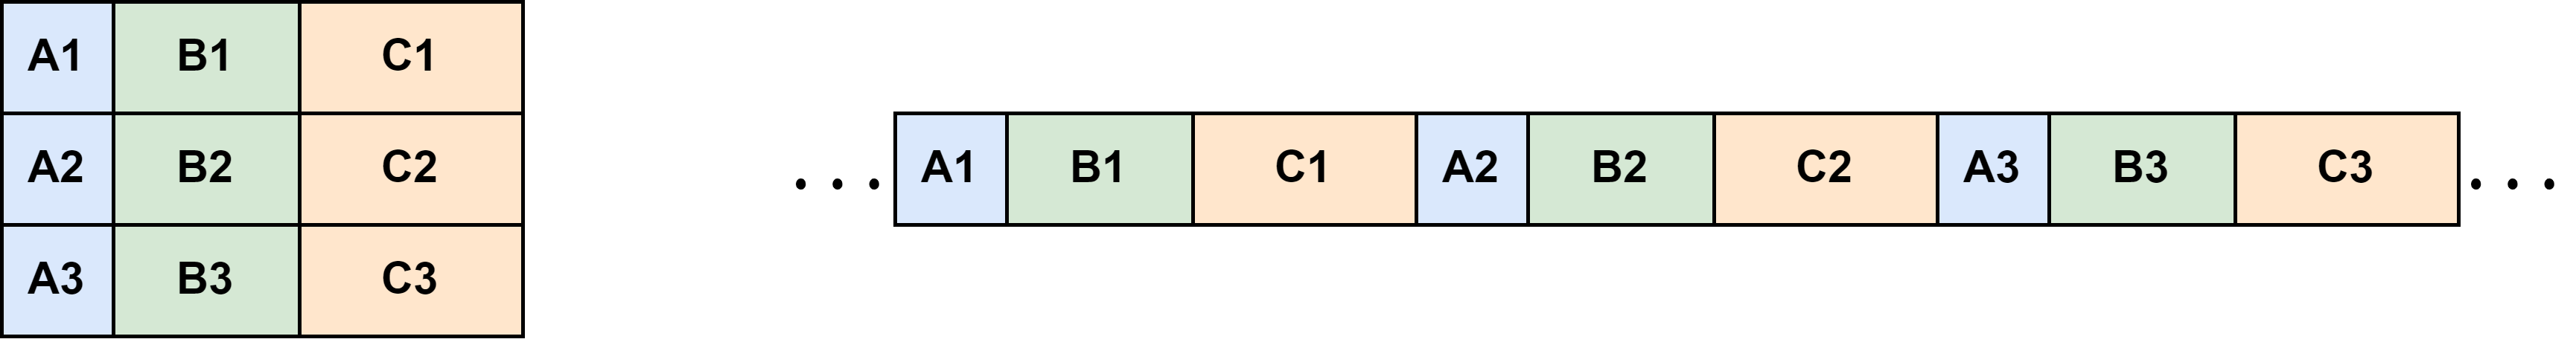
\includegraphics[width=.8\textwidth]{storage/images/nary_layout.drawio.png}
    \end{center}
    \begin{itemize}
        \item Good spatial locality on access to all fields in a tuple.
        \item Works well for lookups and inserts (common in \textit{OTP} where transactions typically run on recent data)
    \end{itemize}
\end{definitionbox}

\begin{definitionbox}{Decomposed Storage}
    Each field of the tuple is stored in a separate array.
    \begin{center}
        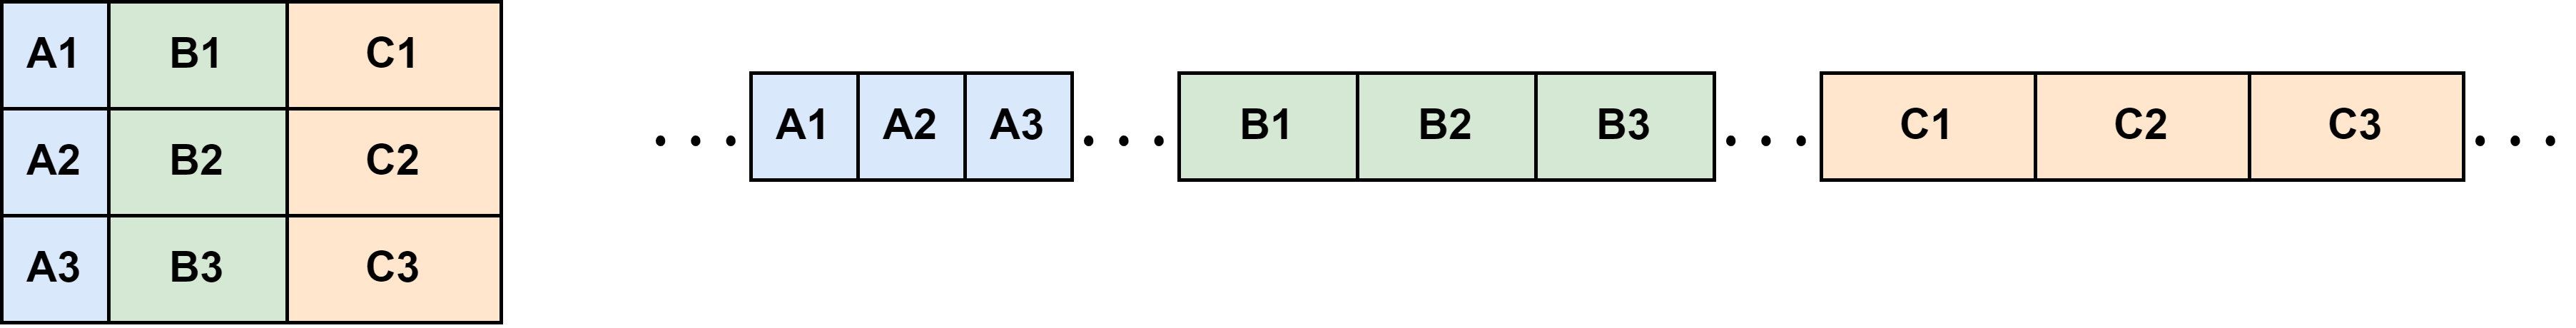
\includegraphics[width=.8\textwidth]{storage/images/decomposed_layout.drawio.png}
    \end{center}
    \begin{itemize}
        \item Good spatial locality when accessing one field of many tuples.
        \item Requires tuples to be reconstructed.
        \item Works well for scan-heavy queries (common in \textit{OLAP} - aggregate, join and filtering)
    \end{itemize}
\end{definitionbox}

\begin{definitionbox}{Delta/Main}
    A hybrid of \textit{n-ary} and \textit{decomposed} storage.
    \begin{center}
        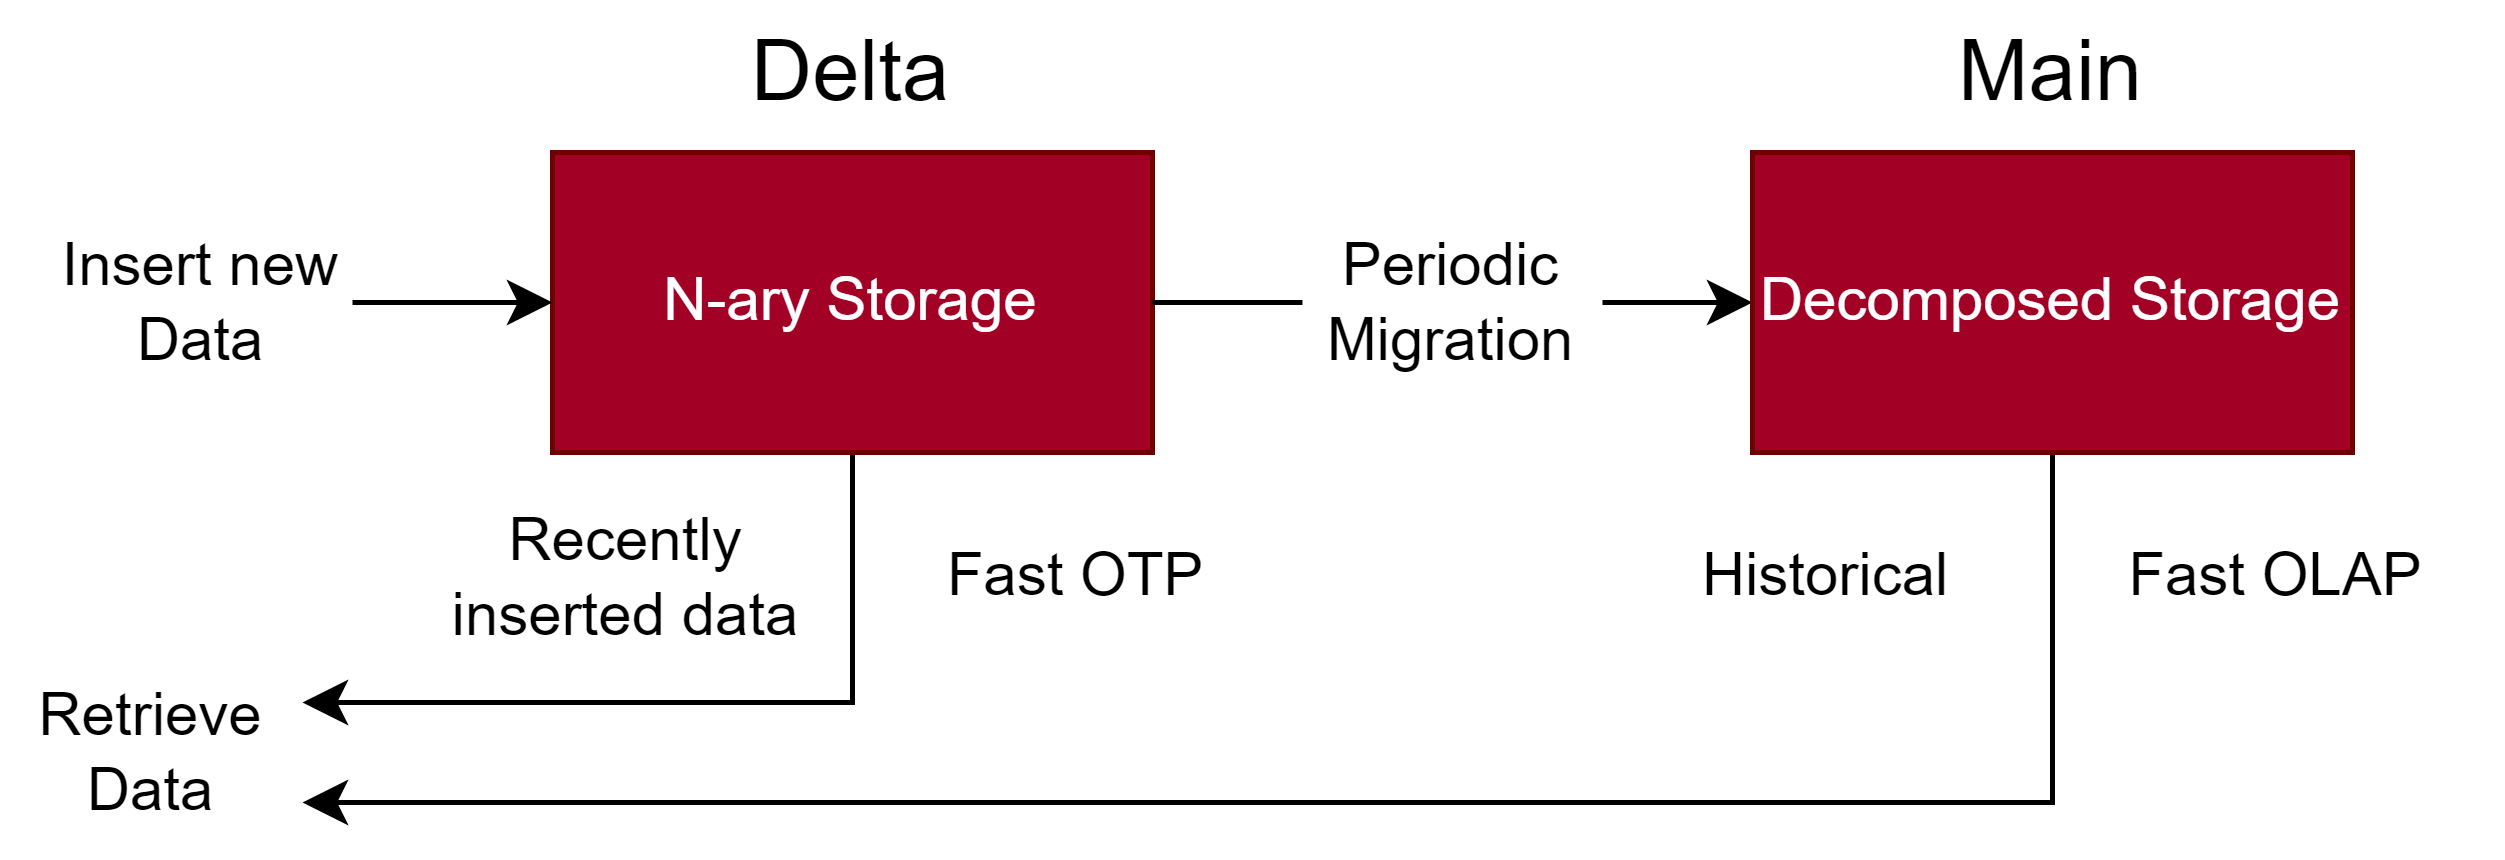
\includegraphics[width=.8\textwidth]{storage/images/delta_main.drawio.png}
    \end{center}
    \begin{itemize}
        \item Complicates some operations (e.g lookups)
        \item Regular migrations can reduce database availability at some points (lock up table to merge)
        \item Can be implemented as a pattern using two separate DBMS (transactional system and data warehouse).
    \end{itemize}
\end{definitionbox}

    
\subsection{Catalog}
\begin{definitionbox}{Catalog}
    Keeps track of database structure (tables, view, indexes etc) and metadata (e.g which tables are sorted, dense)
\end{definitionbox}

\begin{definitionbox}{Dense}
    Records are both sorted and consecutive (e.g $3,4,5$) in some field. Given fixed-size records and the minimum value, records can be looked up in constant time. 
\end{definitionbox}

\subsection{Disk Storage}
\begin{definitionbox}{Buffer Manager}
    Manages disk-resident data and manages data transfer to \textit{pages} in memory.
    \begin{itemize}
        \item Unstructured files $\to$ structured tables
        \item Ensures fixed size for files.
        \item Safely writes data to disk when necessary (to ensure durability).
    \end{itemize}
\end{definitionbox}

\begin{definitionbox}{Unspanned Pages}
    Records only allocated on the page is there is space.
    \begin{center}
        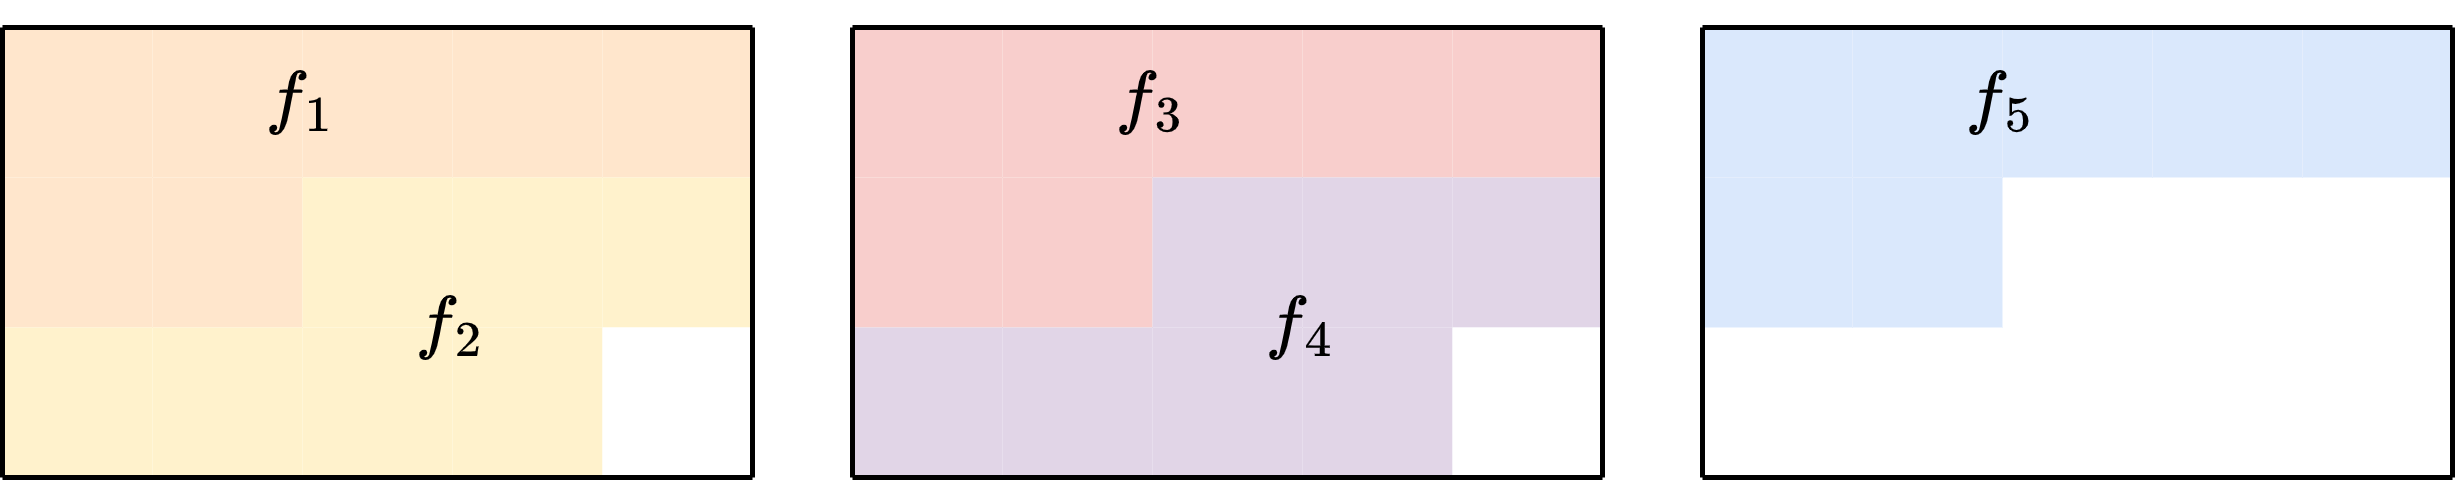
\includegraphics[width=.8\textwidth]{storage/images/unspanned_page.drawio.png}
    \end{center}
    \begin{itemize}
        \item Space wasted (larger as tuple size increases)
        \item If the record size $>$ page size, it is not possible to use this strategy
        \item Assuming there is a know fill factor (number of tuples allocated to each page) we can get fast random lookup for the page a variable size tuple is on.
        \item If records are variable size, no constant time random access within a page.
    \end{itemize}
\end{definitionbox}

\begin{definitionbox}{Spanned Pages}
    Records placed across page boundaries.
    \begin{center}
        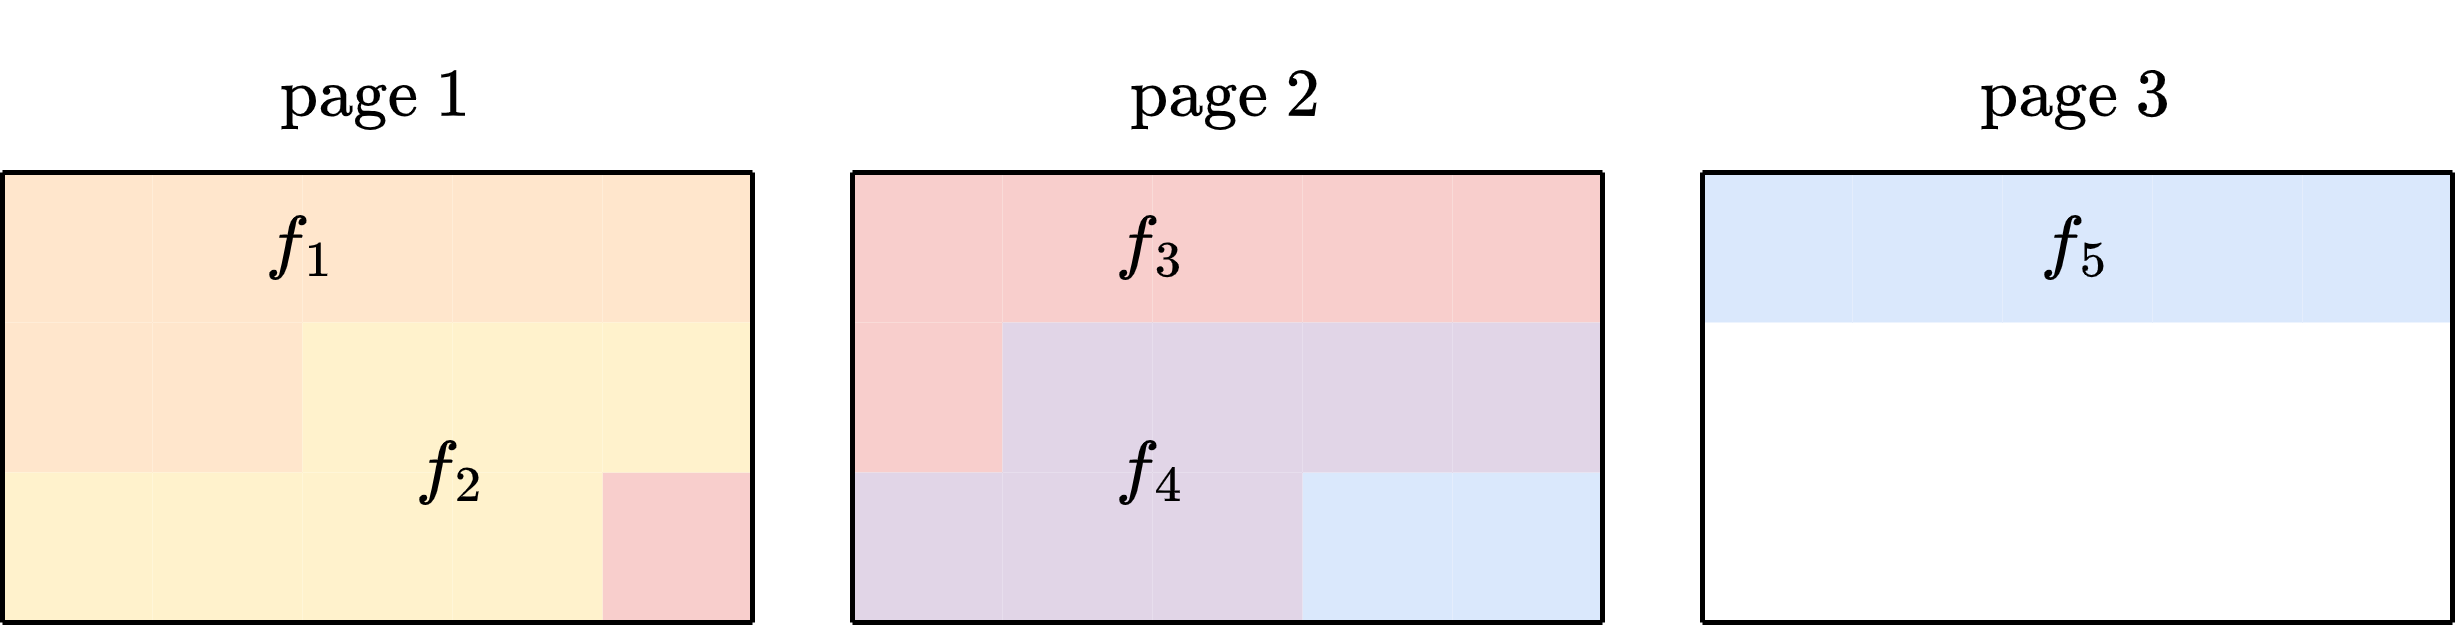
\includegraphics[width=.8\textwidth]{storage/images/spanned_page.drawio.png}
    \end{center}
    \begin{itemize}
        \item Minimises wasted space
        \item Supports very large record sizes (larger than a page)
        \item Complex to implement, and reduced random access performance (with variable size tuples we cannot determine the page a tuple is on in constant time)
        \item If records are variable size, no constant time random access within a page.
    \end{itemize}
\end{definitionbox}

\begin{definitionbox}{Slotted Pages}
    To allow faster/constant time lookup for variable size records.
    \begin{center}
        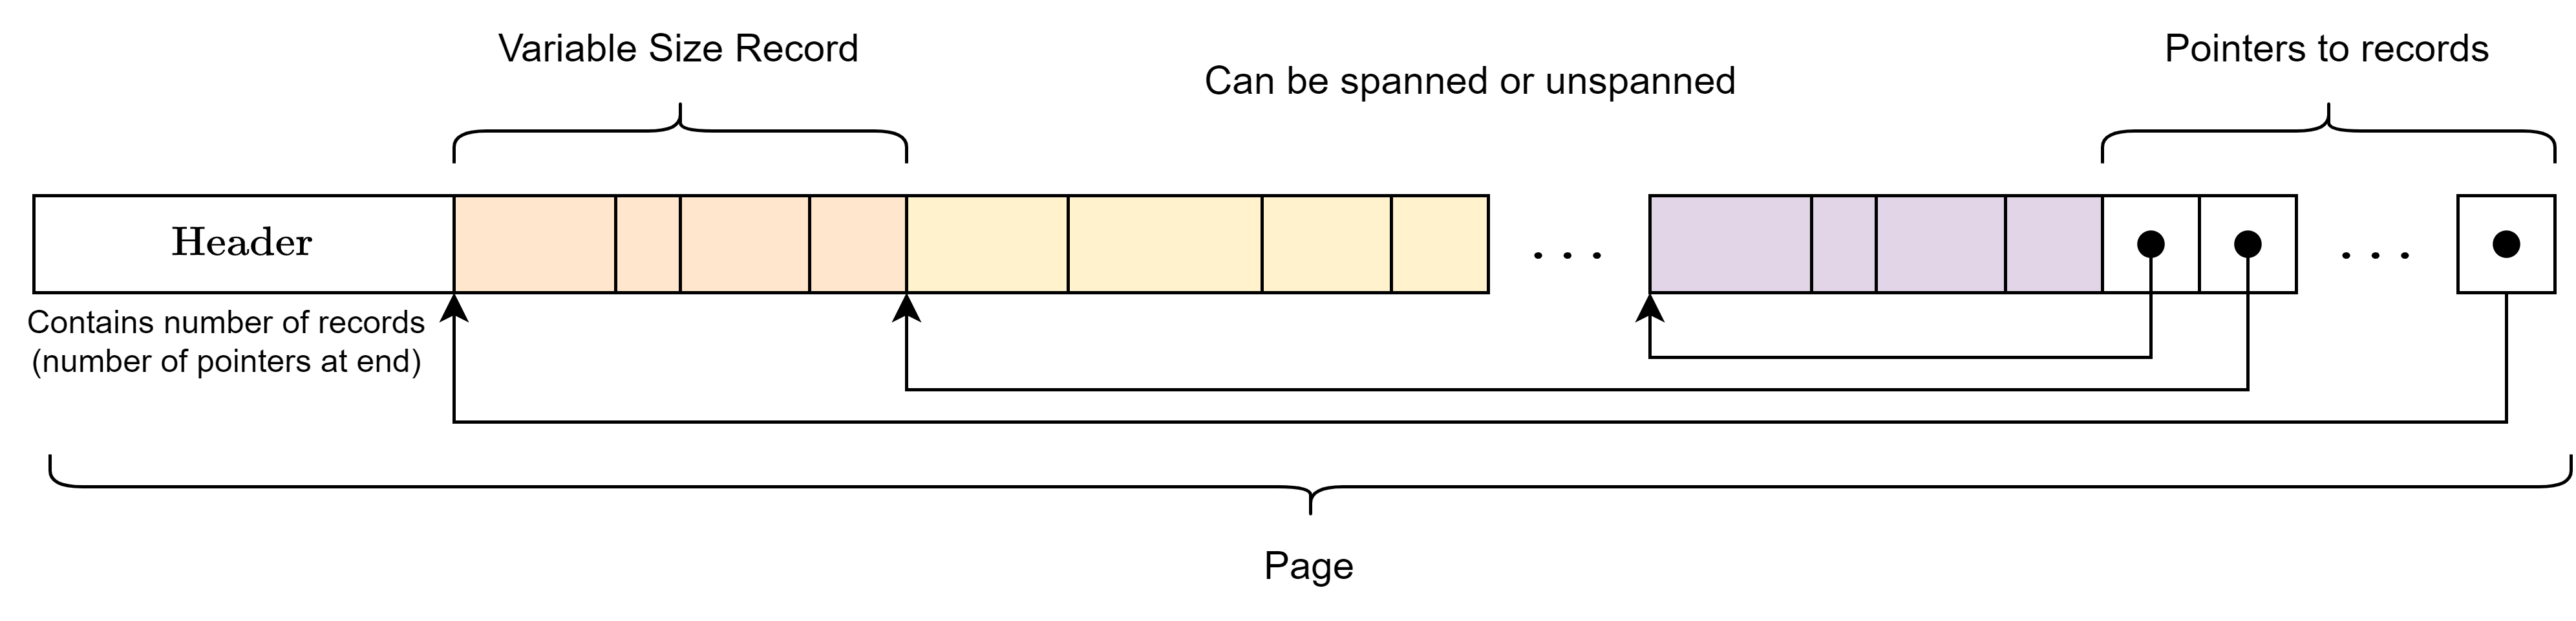
\includegraphics[width=.8\textwidth]{storage/images/slotted_pages.drawio.png}
    \end{center}
    Header stores number of records, index of record used to look-up pointers at the end of the page which are dereferenced to get the record.
\end{definitionbox}

\begin{definitionbox}{Dictionaries}
    Rather than store data (particularly variable-size) in-place it is allocated elsewhere, and a pointer used.
    \begin{center}
        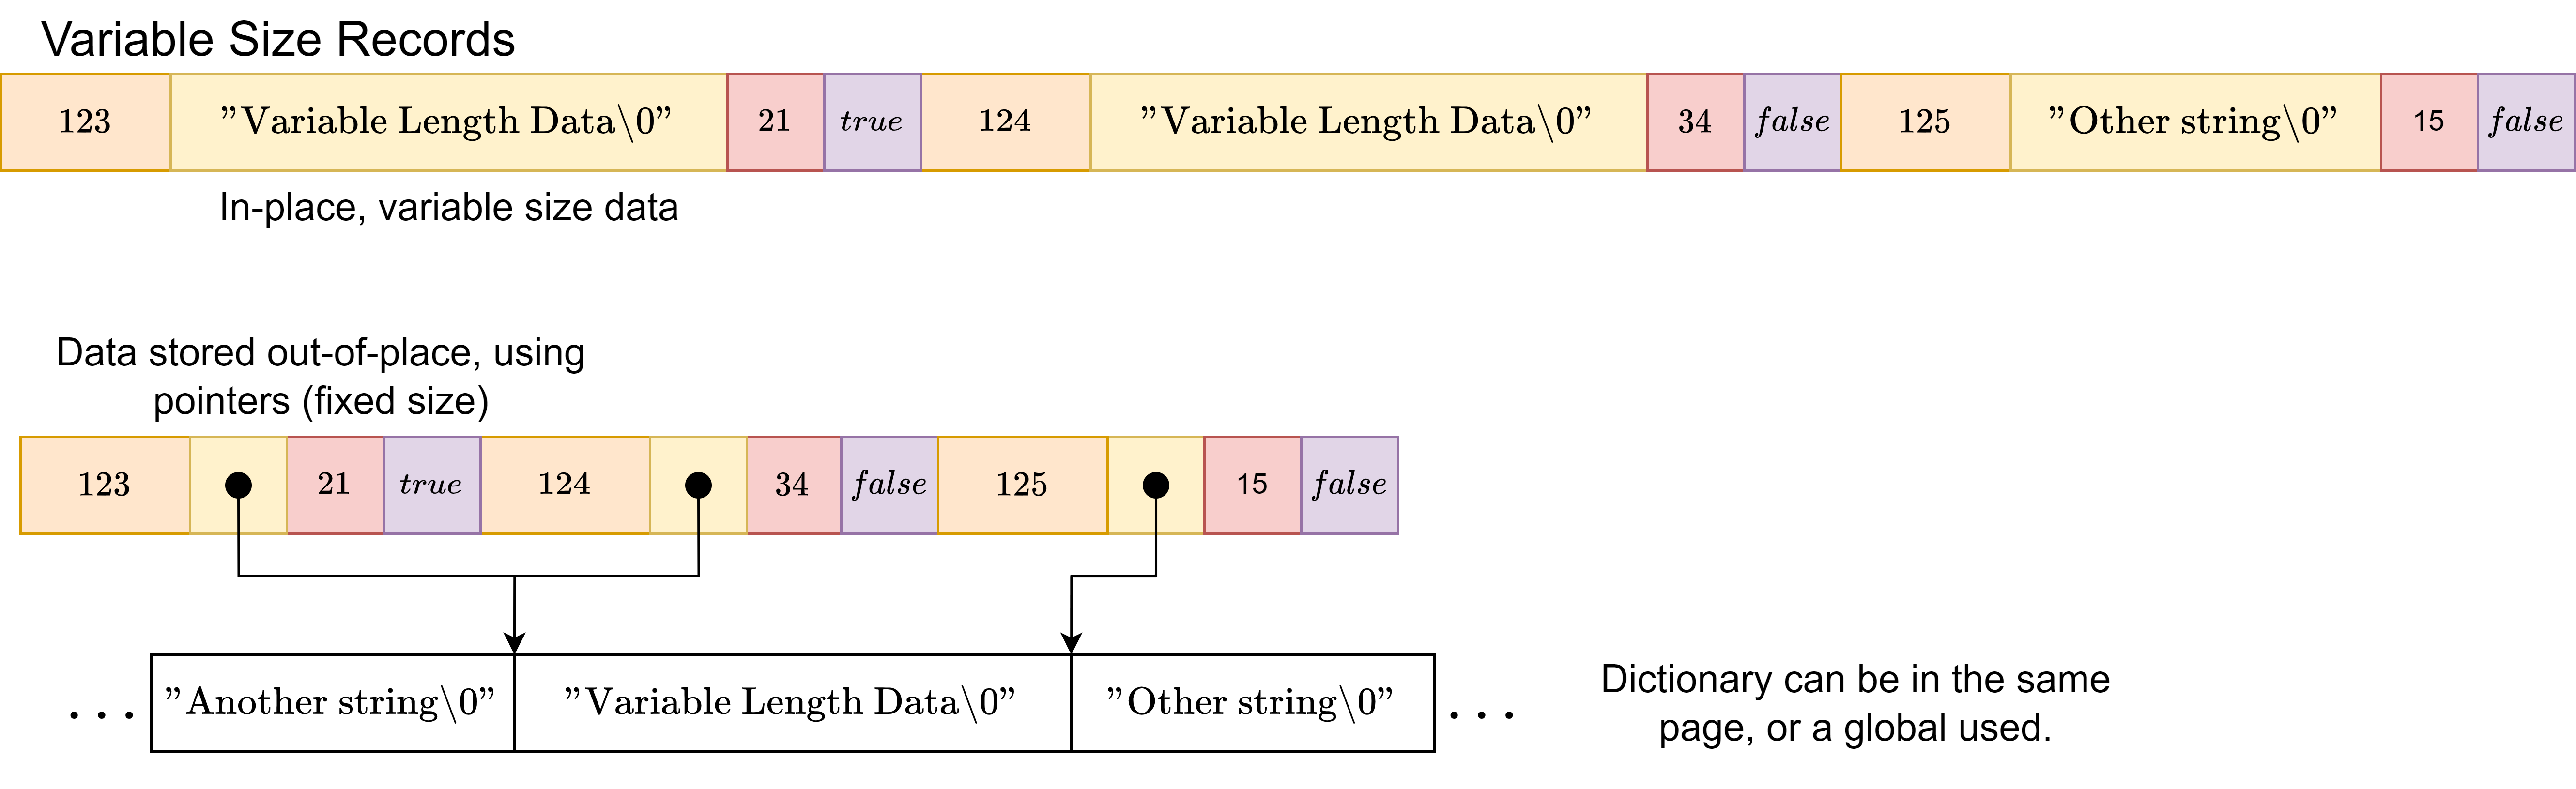
\includegraphics[width=.8\textwidth]{storage/images/dictionary_layout.drawio.png}
    \end{center}
    \begin{itemize}
        \item Can eliminate duplication (duplicate attributes point to the same data)
        \item Need to be careful about managing space (e.g periodically removing unused dictionary entries / garbage collection)
        \item Can reduce spatial locality (record points to non-adjacent dictionary entry), but can (sometimes) improve temporal (same dictionary value accessed many times from many records) 
    \end{itemize}
    \begin{center}
        \begin{tabular}{l p{.8\textwidth}}
            \textbf{In-Page} & Dictionary accesses from within the page do not require other pages to be loaded. Globally more duplicates may exist \& fewer records can be held per page. \\
            \textbf{Global} & A large global dictionary is used (access from other pages require loading). \\
        \end{tabular}
    \end{center}
\end{definitionbox}

\begin{examplebox}{Lookups}
    Access latencies to elements in a table are modelled as follows:
    \[\begin{matrix*}[l]
        n & \text{Access a (32 bit) word for the first time} \\
        m & \text{Access an adjacent word to the last accessed word} \\
        p & \text{Access a previously accessed value} \\
    \end{matrix*} \text{ where } n > m > p\]
    \unfinished
\end{examplebox}

\section{Example Sketch Implementation}
\unfinished

